\documentclass{article} % paper and 12pt font size


\usepackage{amsmath,amsfonts,amsthm} % Math packages
\usepackage{lipsum}
\usepackage{graphicx}

\setlength\parindent{0pt} 

%----------------------------------------------------------------------------------------
%	TITLE SECTION
%----------------------------------------------------------------------------------------

\newcommand{\horrule}[1]{\rule{\linewidth}{#1}} % Create horizontal rule command with 1 argument of height

\title{	
\normalfont \normalsize 
\textsc{Cornell University, INFO/CS 4740: Introduction to Natural Language Processing, Spring 2015} \\
\horrule{0.5pt} \\[0.4cm] % Thin top horizontal rule
\huge PA 1: Language Modeling \\ % The assignment title
\horrule{2pt} \\[0.5cm] % Thick bottom horizontal rule
}
\author{Sofonias Assefa (saa237), La Vesha Parker (ldp47),\\
Alec Sokol (azs8), Nicolas Vera (nmv29)}
\date{\normalsize\today} % Today's date or a custom date
\begin{document}

\maketitle % Print the title

\section{Preprocessing}
\subsection*{Question 1}

\textbf{Give an overview of what you did, explaining any decisions you've made. (E.g. Did you throw away any part of the text? What was considered a word token? Why?)}
\\

% Our answer
We have structured every token in the emails as a custom Unigram object. Our unigram object stores all of the important data that we derive from a token in an email.\\
\begin{center}
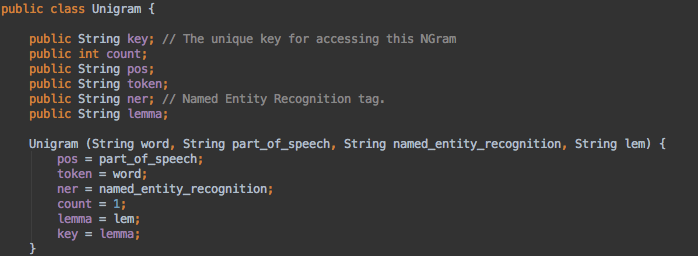
\includegraphics[width=1.0\textwidth]{images/unigram.png}
\textit{An excerpt from the Unigram class.}
\end{center}
We used the Stanford NLP parser to tokenize the emails. Our tokenizing can be broken into separate sections:\\
\begin{itemize}
\item POS Tagging and Lemmatizing:\\
The part-of-speech tags for each of the tokens in our dataset is used very heavily in our classification. In addition to storing the token as it appears in the email, part-of-speech tag, appearance count, and lemma of a given token instantiated as a Unigram, we always reference that Unigram using a key that is formed as "<lemma> <part-of-speech tag>". Therefore, whenever we try to compare a new token against our training models, we are really comparing the lemmatized version of the token along with its part-of-speech tag to the training models. This better maintains the intended use of the tokens in the original emails. and leads to a higher prediction accuracy.
\item Removing case:\\
Simply casting all email content to lower case drastically decreased the number of tokens in our models and increased our social-relationship prediction accuracy on the validation set by 2\%. We found that proper nouns were still classified as such, even with the case removed (i.e. "Natalie" and "natalie" are both parsed as \texttt{NNP}). That was our main concern when we decided to test our predictions in a case-insensitive environment, so that was positive reinforcement on our decision to use a single case throughout our classification process.
\end{itemize}

In terms of text that we "threw away," a major simplification we used was that of numbers. We achieved a 3\% increase in accuracy of our predictions when we simplified the way we used numbers. Upon reviewing the numeric tokens found in the training and validation sets, we derived five useful classifications of numbers. The classes are as follows:\\
\begin{itemize}
\item Phone Numbers:\\
We accept the three most popular formats for phone numbers: 
	\begin{itemize}
	\item Phone numbers separated by hyphens (-), periods (.), or spaces: XXX-XXX-XXXX, XXX.XXX.XXXX, XXX XXX XXXX
	\item Phone numbers with no separators: XXXXXXXXXX
	\item Phone numbers with the area code emphasized: (XXX) XXX-XXXX
	\end{itemize}
\item Time:\\
The majority of times in the data set followed the pattern "HH:MM," where "H" is an hour and "M" is a minute. We allow for single-digit specification of hours and minutes as well.
\item Date:\\
We process dates of the form MM/DD/YYYY, as is the format for the majority of dates.
\item Zipcode:\\
Either 5 or 9 numeric characters together, in proper zipcode format
\item General Number:
Anything that is numeric, but does not fit the above categories. i.e. "1,234,567,910", "1111111", "+11111", etc.
\end{itemize}

Each of the cases above for numeric tokens were then used to represent the token itself. In that way, a number like "1,234,567,910" is recognized by our system as a "generic\_number", instead of as "1,234,567,910". This allowed us to better group similar numeric tokens, instead of depending heavily on the actual values of the numeric tokens. 

\section{Unsmoothed n-grams}
\subsection*{Question 2}

\textbf{Give an overview of what you did, explaining any decisions you?ve made. (E.g. Did you keep the capitalization? Which punctuation marks did you keep, if any?)}
\\

% Our answer

\lipsum[2] % Dummy text

\subsection*{Question 3}

\textbf{List 10 most frequent n-grams for each of the 6 models.}
\\

Written as $<$N-gram$> <$count$>$:\\

\textsc{Up-speak Unigram Model}\\
\begin{enumerate}
\item $<$s$>$ 10940
\item $<$/s$>$ 10940
\item . 4222
\item the 3838
\item , 3224
\item to 2727
\item be 2662
\item \texttt{general\_number} 2432
\item and 1630
\item of 1506
\end{enumerate}

\textsc{Down-speak Unigram Model}\\
\begin{enumerate}
\item $<$s$>$ 10936
\item $<$/s$>$ 10936
\item . 4045
\item the 3845
\item , 3202
\item be 2892
\item to 2375
\item \texttt{general\_number} 1722
\item you 1520
\item I 1504
\end{enumerate}

\textsc{Up-speak Bigram Model}\\
\begin{enumerate}
\item . $<$/s$>$ 4191
\item , $<$/s$>$ 613
\item $<$s$>$  I 571
\item \texttt{general\_number} $<$/s$>$ 509
\item $<$s$>$  the 413
\item $<$s$>$  please 403
\item of the 380
\item $<$s$>$ \texttt{general\_number} 316
\item in the 300
\item will be 297
\end{enumerate}

\textsc{Down-speak Bigram Model}\\
\begin{enumerate}
\item . $<$/s$>$ 4027
\item , $<$/s$>$ 586
\item $<$s$>$ I 528
\item $<$s$>$ the 484
\item $<$s$>$ please 446
\item of the 384
\item if you 384
\item \texttt{phonenumber} $<$/s$>$ 370
\item will be 366
\item $<$s$>$  thanks 351
\end{enumerate}

\textsc{Up-speak Trigram Model}\\
\begin{enumerate}
\item $<$s$>$  Vince $<$/s$>$ 208
\item \texttt{general\_number} . $<$/s$>$ 204
\item $<$s$>$  Shirley , 199
\item Shirley , $<$/s$>$ 196
\item $<$s$>$  \texttt{general\_number} . 157
\item $<$s$>$  \texttt{date} \texttt{time} 129
\item \texttt{general\_number} \% $<$/s$>$ 117
\item $<$s$>$  please , 111
\item today \texttt{general\_number} $<$/s$>$ 109
\item $<$s$>$  if you 105
\end{enumerate}

\textsc{Down-speak Trigram Model}\\
\begin{enumerate}
\item $<$s$>$  Vince $<$/s$>$ 208
\item \texttt{general\_number} . $<$/s$>$ 204
\item $<$s$>$  Shirley , 199
\item Shirley , $<$/s$>$ 196
\item $<$s$>$  \texttt{general\_number} . 157
\item ) . $<$/s$>$ 141
\item $<$s$>$  \texttt{date} \texttt{time} 129
\item \texttt{general\_number} \% $<$/s$>$ 117
\item $<$s$>$  please , 111
\item today \texttt{general\_number} $<$/s$>$109
\end{enumerate}


\subsection*{Question 4}

\textbf{Compare the n-grams. What do they tell you about the respective
models?}
\\

The start and end tags are prominent in each model.

There is an interesting similarity in the unigram models, as they pretty much match expectations in terms of most frequently occurring words and punctuation marks. After the start and end tags, very common punctuation marks like the period and comma are highly ranked (ranked 3 and 5 in both models, respectively). As expected, "the" is the most frequently occurring word as well. The other four words are all generally considered stop words, and the last type of  token in the top 10 is a \texttt{general\_number}, which is to be expected seeing as the email correspondents "talk numbers" frequently.\\

The slight change between the unigram and bigram models is interesting, because the bigram models start to incorporate common ways of starting an email or sentence, such as a salutation or term of respect. It also contains commonly used phrases such as partial-prepositional phrases like "of the" and "in the". Again, phrases containing the word "the" are highly ranked, no doubt a byproduct of "the"'s rank in the unigram models. A more interesting number type, \texttt{phone number}, also makes an appearance in the down-speak bigram model.

Between the bigram and trigram models, number types make even more of an appearance, with more combinations of \texttt{general\_number}s with various popular punctuation marks. It is also interesting to note that all of the top 10 phrases for both the up-speak and down-speak trigram models contain either the start tag ($<$s$>$), end tag ( $<$/s$>$), or both.

The form of changes between up and down-speak for the same N-Gram model were not as clear as the differences for different values of $N$. If we were to expand the selection to the top 30 or so N-Grams, we would more likely see a greater difference in speak type, especially in the trigram model.

\section{Random sentence generation}
\subsection*{Question 5}

\textbf{Give an overview of what you did, explaining any decisions you've made.}
\\

The Random Sentence Generator (RSG) is written in \texttt{RSG.java}. Running the main method will produce 20 random sentences for each of the 6 language models (unigram, bigram, trigram; and downspeak, upspeak for each).\\

\texttt{RSG.java} requires the 6 \texttt{.json} files in the \texttt{models} directory. These files contain, for each of the language models, information about the n-grams including the numbers of occurrences for each.\\

It is best to describe how the RSG uses the unigram models first, since the use of the bigram and trigram models builds upon it. First, the file containing the unigrams and their counts is read in. The values are inserted to a Java ArrayList of Strings. Each unique unigram is inserted into the ArrayList an amount of times equal to its count. For example, if our n-gram information tell us:\\

\texttt{hello 3\\
there 1\\
my 2\\
friend 1}\\

the resulting  \texttt{ArrayList} will be:\\

\texttt{["hello", "hello", "hello", "there", "my", "my", "friend"]}\\

This approach was taken in order to intuitively implement distributed probability. Since  \texttt{ArrayList} is an indexed data structure, picking a random index results in selecting a random word. The more times that word appears in the  \texttt{ArrayList}, the more likely it is to be selected. Although doing this increases the running time, the extent to which it does is fairly negligible. Speed was not of concern for this project and the sentences will print out in a matter of seconds.\\

For the unigram model, $N - 0$ here is equal to 0, so each word is picked without consideration of the previous word. A String randomSentence is initialized with the start-of-sentence tag  \texttt{$<$s$>$} and has each new random word appended to it. It is returned once the end-of-sentence tag  \texttt{$<$/s$>$} has been appended or  \texttt{SENTENCE\_MAX} has been reached.\\

Generating sentences with the bigram models requires the consideration of the previous word. The RSG looks at the previous word and then reads in the bigram model file, adding to an  \texttt{ArrayList} only the bigrams that begin with the previous word. This is done in the same fashion that the unigrams were stored in (with each bigram being inserted as many times as its respective count, so that distributed probability is applied). Again, this is done repeatedly until the sentence comes to an end.\\

For the trigram models, the previous two words of the sentence being generated need to be considered. The first iteration is done exactly the same as with the bigram models because at the beginning of the sentence, there is only one previous word (the start-of-sentence tag  \texttt{$<$s$>$}). After that, new random words are picked just as they were using the bigram models but instead, we look at the previous two words. That is to say, each new word selected is the third word in the randomly selected trigram whose first two words are the previous bigram.\\

\subsection*{Question 6}

\textbf{Provide 5 example sentences each of the 6 models.}
\\
\textbf{Unigram downspeak:}\\

\texttt{$<$s$>$ CORP subordinate cosider DuPont tool obtain Bun '03 Zipper fare fishing cover Conoco perhaps Florida e-mail think feel...\\
$<$s$>$ PPL Environmental move Lender Janel ten Kathryn Rhodes case sale White Alexis percentage El partial inside relevant belong deliver 9-apr-01...\\
$<$s$>$ condition paymet value mild tetracycline grandmother Fri. discourage quantity give reserve hearing...\\
$<$s$>$ want support nerveousness tue adupont@pdq.net rp Treating timekeeper Kerry proposal new E.W.S. chunck agency...\\
$<$s$>$ Mids Badu Milwaukee responsible Callans confidentiality 11/28/01 American 11mm acquaint...}\\

\textbf{Unigram upspeak:}\\

\texttt{$<s$> combustor number diversity = winner Peaks Video Tamsin advocacy line Wisconsin...\\
$<s$> NYSE side discount Service move Casper function DPR library Causey co2 Load.Load...\\
$<s$> location modify rule program Kong boat nondiscrimination Implementation summer-season additionally...\\
$<s$> pre important High sponsor limit struggle free HPL Association net clay file some plan...\\
$<s$> compromise Re McCarty interference abou 713 410 5396 head Supatgiat UK Calcasieu...}\\

\textbf{Bigram downspeak:}\\

\texttt{$<$s$>$ for next week start Mid East Power $<$/s$>$\\
$<$s$>$ no make sure that Kenneth Lovejoy have overall responsibility roll over Pease St. to use only if you , and b confirm as with yourselve $<$/s$>$\\
$<$s$>$ I 's credit term this print - there be a be handle in late intelligence support from a and the spreadsheet . $<$/s$>$\\
$<$s$>$ coordination will let later $<$/s$>$\\
$<$s$>$ I think the scope of the guy get the attorney who complain or to I just go target . $<$/s$>$}\\

\textbf{Bigram upspeak: }\\

\texttt{$<$s$>$ with the be out of the information . $<$/s$>$\\
$<$s$>$ Vince , and first item to I know the please contact $<$/s$>$\\
$<$s$>$ thank you to meet each month be only to the select to have comment $<$/s$>$\\
$<$s$>$ decision , fee privileged to Afghan opposition to legal claim that query to and Fred 's desk to he $<$/s$>$\\
$<$s$>$ Shall we , but I at be change that the golf or clickpaper-related counterparty for the incremental fee a Tentative Business school $<$/s$>$}\\

\textbf{Trigram downspeak:}\\

\texttt{$<$s$>$ I want to make payment directly to we , still we be take at this time of need . $<$/s$>$\\
$<$s$>$ you have any question . $<$/s$>$\\
$<$s$>$ feedback from customer and post on the actual date of the email I send a email to Kim Hillis be make progress , and wptf be go -rrb- . $<$/s$>$\\
$<$s$>$ standardize market , and be not move as quickly due to operational constraint on the website . $<$/s$>$\\
$<$s$>$ now let 's make it a 2:30 $<$/s$>$}\\

\textbf{Trigram upspeak:}\\

\texttt{$<$s$>$ Tuesday , July 12 , 2001 $<$/s$>$\\
$<$s$>$ Rick will hold a conference call schedule for Thursday 's call with John Lavorato and Louise , $<$/s$>$\\
$<$s$>$ I be not correct in TMS do not focus on achieve the objective of Enron . $<$/s$>$\\
$<$s$>$ sorry for the extra time for the last transaction that John have execute be Enron 's message and purpose . $<$/s$>$\\
$<$s$>$ Honey Baked ham $<$/s$>$}


\subsection*{Question 7}

\textbf{Compare the sentences. What do they tell you about the respective models?}
\\

The sentences generated using the unigram models look truly random and are notably less intelligible than those generated by the other models. Sentences turned out to be quite long, so setting a sentence maximum length was necessary. This is likely due to the fact that previous words weren't considered, and so sentences did not tend to come to an end naturally like the sentences generated by the other models seemed to do. \\

The bigram models provided more intelligible sentences. Sentences came to natural ends. Familiar phrases such as "thank you" "make sure" made appearances, as well as syntactically correct phrases such as "please" followed by a verb. Additionally, a distinction began to appear between upspeak and downspeak. Upspeak seemed to contain more interrogative language such as "please" and "shall we" than the downspeak sentences did.\\

The trigram models produced more syntactically as well as semantically correct sentences than the other models. Longer phrases with discernible meaning appeared, such as "Rick will hold a conference call," "sorry for the extra time," and "I want to make payment directly." Overall, there was a direct relationship between N and the quality of the sentences in terms of syntax and comprehensibility.


\section{Unknown Word Handling and Laplace Smoothing}

\subsection*{Question 8}

\textbf{Give an overview of what you did, explaining any decisions you?ve made. (E.g. How are you handling the unknown words and why?)}
\\

We initially implemented add-one smoothing (mostly due to the fact that it was a required part of the assignment), but we soon realized that it was largely inaccurate. Because of some feedback on Piazza about the inaccuracy of Kneser-Ney Discounting for this particular data set, we opted to implement Good-Turing Smoothing as our main smoothing method.\\

We initially tried to use a combination of the various implemented smoothing methods (unigram, bigram, trigram add-on and unigram, bigram, and trigram Good-Turing) when classifying an email as up or down. This approach, however, led to largely inaccurate results. The add-one smoothing methods and the less complex N-gram models using Good-Turing Smoothing were just too unpredictable and ineffective at classifying emails, which was decreasing the overall effectiveness of the classifier. In the end, we opted with using the trigram Good-Turing model on it's own, and this drastically increased our classification ability.\\

Unknown words are handled using the add-one method so that they had a nonzero probability. This was used in conjunction with Good-Turing smoothing as listed above. Depending on the type of unknown string, we used more complex classification methods. More specifically, times, dates, zip-codes, and phone numbers all had their own unique classification. These were kept separate and handled differently from the more general group of all unknown words.

\section{Perplexity}

\subsection*{Question 9}

\textbf{Provide the perplexities of the 6 models with respect to the respective validation set.}
\\

% Our answer
Our perplexity values were computed using Laplace smoothing, and a log transformation to prevent overflow. The final formula used for the computation was:
$$
- \frac{1}{N} \sum\limits_{i = 0}^N log(P(W_i|W_{i - (n-1)},...,W_{i-1})
$$
Using Laplace smoothing, our calculated log perplexities are as follows: \\

\begin{center}
\begin{tabular}{ l | r}
	\hline
		Validation Set & Log Perplexity \\
	\hline
		Upspeak Unigram & 6.47740934048416 \\
		Downspeak Unigram & 6.597998169837239 \\
		Upspeak Bigram & 7.331584597485108 \\
		Downspeak Bigram & 7.43914010534209 \\
		Upspeak Trigram & 7.543225576737731 \\
		Downspeak Trigram & 7.7767272961338145 \\
	\hline
\end{tabular}
\end{center}

\subsection*{Question 10}

\textbf{Compare the perplexities. Are they consistent with your expectations? Why or why not?}
\\

The perplexity values (relative to each other) as we expected them to be. In both upspeak and downspeak, the perplexity of the trigram set > perplexity of the bigram set > perplexity of the unigram set.

For n-gram sets, the size of a set's potential vocabulary grows exponentially with n. Therefore, we can definitely expect more sparsity in higher n-gram models. This difference should be visible in the perplexities of independent validation sets. Indeed, the table above is consistent with this differences in perplexities.


\section{Social Power Relationship Prediction}


\subsection*{Question 11}

\textbf{Explain how you train your the language models. (Which smoothing method? Are you doing any special preprocessing?)}
\\

Training happens independently for our six models: upspeak unigram, downspeak unigram, upspeak bigram, downspeak bigram, upspeak trigram, downspeak trigram. Each model contains a set of all of the word lemmas encountered in its corresponding training set, and extra information such as part of speech, frequency in the training set, and word type itself. Word lemmas are used here instead of the actual tokens to better counter sparsity and simplify the vocabulary we are working with.

We preprocess our training data by ......

All six models use Good-Turing smoothing.

\subsection*{Question 12}

\textbf{Explain how you classify each email as UPSPEAK or DOWNSPEAK, given the probabilities computed by using the language models.}

For both the test set and validation sets, classification happens once at the sentence level, and then again at the email level. Each sentence is classified independently using three different trained models: unigram model, bigram model, trigram model. 

Each sentence is classified with the most common speak type from three models. Each email is classified with the most common speak type from all of its sentences.

\subsection*{Question 13}

\textbf{How well does your classifier perform?}

Our classifier achieves an accuracy of 40$\%$ on the provided test set.

\end{document}
